\documentclass[12pt,a4paper]{article}
\usepackage[utf8]{inputenc}
\usepackage[spanish]{babel}
\usepackage{amsmath}
\usepackage{amsfonts}
\usepackage{amssymb}
\usepackage{makeidx}
\usepackage{graphicx}
\usepackage[left=2cm,right=2cm,top=2cm,bottom=2cm]{geometry}

\author{Felipe Alvarado Galicia}
\title{IDENTIFICAR LAS APLICACIONES DE LOS MANIPULADORES PARALELOS}
\date{Profesor:Carlos Enrique Moran Garabito\\
Materia: Cinematica de Robots\\
n de octubre de 2019}

\begin{document}
\maketitle
 
\includegraphics[scale=1]{logo1.png}\\
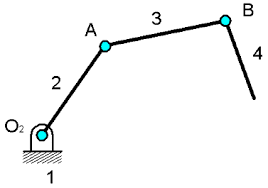
\includegraphics[scale=1]{imag5.png} 
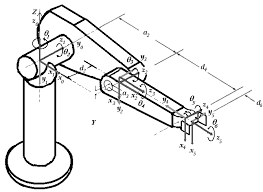
\includegraphics[scale=1]{imag8.png}\\\\\\\\\\\\\\\\\\\\\\\\\\\\\\\\\\\\\\\\\

\tableofcontents
.\\\\\\\\\\\\\\\\\\\\\\\\\\\\\\\\\\\\\\\\\\\\\\\\\\\\\\\\\\\\\\\\\\\\\\\\\\\
\section{Manipulador paralelo:}
Es un dispositivo multifuncional y reprogramable diseñado para mover y manipular materiales, partes o herramientas a través de movimientos programados variables para la realización de una variedad de tareas especificadas.\\
Un robot paralelo está compuesto por una cadena cinemática cerrada, la cual consta de cadenas seriales separadas que conectan al eslabón fijo (plataforma fija) con el efector final o eslabón móvil (plataforma móvil).\\
Los robots también son llamados manipuladores, y ambos términos son manejados en este trabajo.\\
\begin{center}
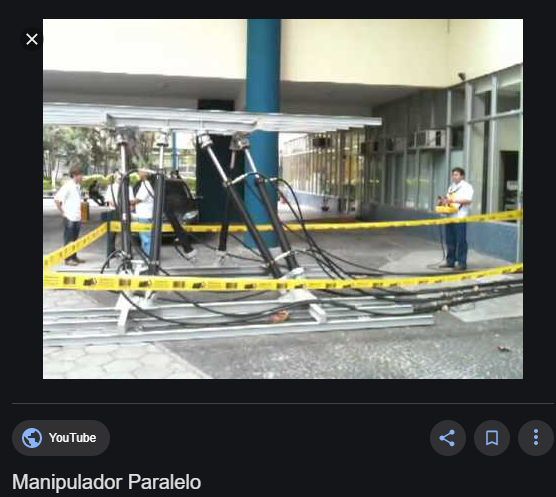
\includegraphics[scale=1]{3.PNG}
\end{center}
.\\\\\\\\\\\\\
\section{Aplicaciones de los manipuladores paralelos} 
Aplicaciones:\\
Este tipo de manipulador presenta grandes ventajas comparado con los manipuladores seriales, como son: mejor estabilidad y precisión, peso ligero, capacidad de manipular cargas relativamente grandes, altas velocidades y aceleraciones, y baja fuerza de actuación.\\

En la actualidad los robots son parte fundamental de nuestra industria, facilitando la ejecución de múltiples tareas, aumentando la precisión del producto final y disminuyendo tiempos de ejecución.\\ Además, son muchos otros los ámbitos en los que los sistemas robóticos modernos colaboran, como pueden ser el sector aeroespacial, diversas aplicaciones médicas, industria de los videojuegos, etc. En particular, los denominados manipuladores paralelos han ido adquiriendo en los últimos años una notable relevancia, existiendo numerosas líneas de investigación y proyectos asociados al estudio y desarrollo de este tipo de robots.\\

Hay diferentes tipos de Manimuladores de paraleos, pero al final todos se rigen por algunas reglas para que se puedan identificar o diferencias de otros tipos de manipuladores.\\
Entre ellos estan los siguientes; \\
\begin{center}
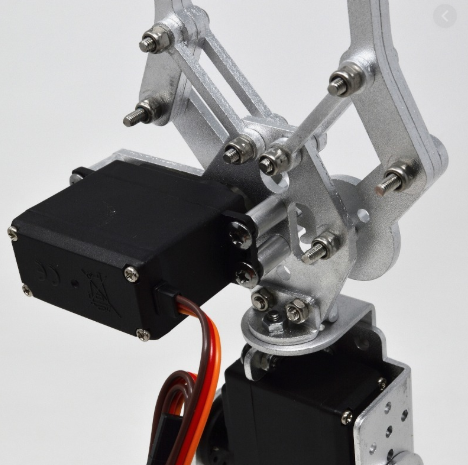
\includegraphics[scale=1.15]{1.PNG}
\end{center}
.\\\\
Otras de las aplicaciones de los robots paralelos se han venido empleando para distintas tareas como en simuladores de vuelo, máquinas caminadoras, dispositivos de máquinas–herramientas, micro manipulación a alta frecuencia (telescopios), asi tambien como en las empresas refresqueras y de comida, en procesos de empaquetamiento, analisis de dimenciones para calidad del producto y recientemente para tareas de ensamble.
\begin{center}
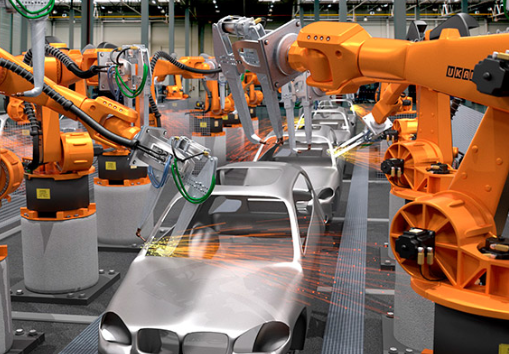
\includegraphics[scale=1.28]{4.PNG}
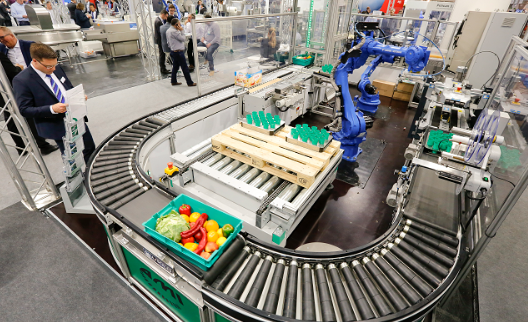
\includegraphics[scale=1.23]{7.PNG}
\end{center}
\section{Claificación}
A) PLANARES:\\
Llamados también robots móviles que navegan en el plano, bastaría con un espacio de dimensión tres para especificar la posición y el ángulo de orientación.\\
B) ESFÉRICOS:\\
Se caracteriza por dos articulaciones de rotacion y una prismática, las variables articulares expresan la posición del extremo del tercer enlace de coordenadas polares.\\
C) ESPACIALES:\\
También se pueden clasificar de acuerdo a sus características estructurales como: simétricos y asimétricos.\\
\begin{center}
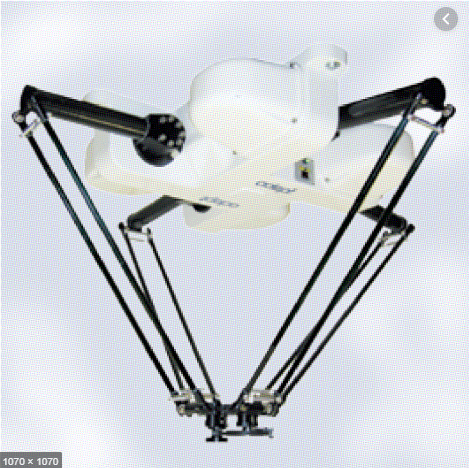
\includegraphics[scale=1]{2.PNG} 
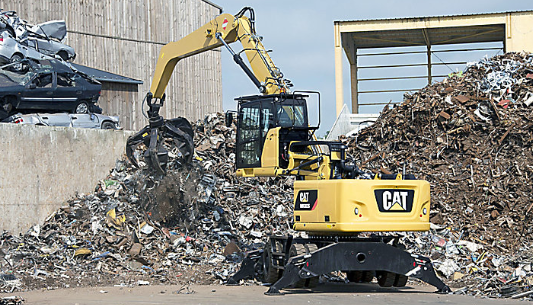
\includegraphics[scale=1.2]{5.PNG} 
.\\
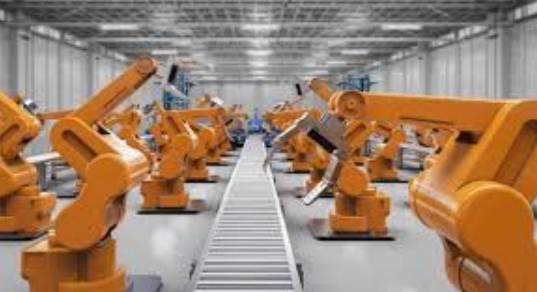
\includegraphics[scale=1.2]{6.PNG}
\end{center}
.\\\\\\\\\\\\\\\\\\\
\section{Bibliography}
https://slideplayer.es/slide/9070603/ \\
https://www.revistadyna.com/busqueda/estado-de-tecnica-de-manipuladores-paralelos-aplicaciones-practicas-y-criterios-cinematicos-de-disen \\



\end{document}